%<dscrpt>Projection stéréographique et équation de Ricatti complexe.</dscrpt>
On considère une équation différentielle
\begin{displaymath}
 z' = 1 + z^2 \hspace{1cm}(1)
\end{displaymath}
Une solution est une fonction définie et dérivable dans un intervalle $I$ de $\R$ et à valeurs \emph{complexes}.
\subsection*{Partie 1. Nature des trajectoires}
\begin{enumerate}
 \item Déterminer les solutions qui sont des fonctions constantes définies dans $\R$.
\item Donner une solution à valeurs réelles en précisant soigneusement son intervalle de définition.
\item Soit $z$ une fonction à valeurs complexes définie et dérivable dans un intervalle $I$ de $\R$. On pose $x=\Re(z)$ et $y=\Im(z)$.
Former un système $(\mathcal S)$ de relations entre $x$, $y$ et leurs dérivées tel que $z$ soit solution de $(1)$ si et seulement si $x$ et $y$ vérifient $(\mathcal S)$.
\item Soit $z$ une solution de $(1)$. Calculer la dérivée de
\begin{displaymath}
 \dfrac{\Im z}{1+|z|^2}
\end{displaymath}
\item \`A toute solution non constante $z$ de $(1)$ définie dans un intervalle $I$, on associe la courbe paramétrée $Z$ telle que, pour tout $t\in I$, $Z(t)$ est le point d'affixe $z(t)$ dans un plan muni d'un repère orthonormé.\newline
On suppose que $0\in I$ avec $z(0)=i\lambda$ pour $\lambda$ réel non nul. Montrer que le support (trajectoire) c'est à dire l'ensemble de points
\begin{displaymath}
 \left\lbrace Z(t), t\in I\right\rbrace 
\end{displaymath}
est inclus dans une courbe géométrique dont on précisera la nature et les éléments caractéristiques en fonction de $\lambda$. Quels sont les points d'intersection de cette courbe avec l'axe $(Oy)$ ?
\end{enumerate}

\subsection*{Partie 2. Expressions des solutions}
On cherche ici à exprimer les solutions de $(1)$ à l'aide de fonctions usuelles.
\begin{enumerate}
 \item 
\begin{enumerate}
\item Déterminer l'ensemble des fonctions à valeurs complexes vérifiant
\begin{displaymath}
 \forall t\in \left] -\frac{\pi}{2} , \frac{\pi}{2}\right[ : z'(t) + 2\tan(t) \, z(t)=0
\end{displaymath}
\item Déterminer l'ensemble des fonctions à valeurs complexes vérifiant
\begin{displaymath}
 \forall t\in \left] -\frac{\pi}{2} , \frac{\pi}{2}\right[ : z'(t) + 2\tan(t) \, z(t) = -1
\end{displaymath}
\end{enumerate}

 \item Soit  $I$ un intervalle inclus dans $\left] -\frac{\pi}{2} , \frac{\pi}{2}\right[$ et contenant $0$.\\ Soit $z$ une solution de $(1)$ définie et dérivable dans $I$ telle que $z(0)=i\lambda$ avec $\lambda$ réel non nul.
\begin{enumerate}
 \item Montrer que  $z(t)\neq \tan t$ pour tout $t\in I$.
\item Former une équation différentielle dont la fonction définie dans $I$ par
\begin{displaymath}
 t \rightarrow \dfrac{1}{z(t)-\tan(t)}
\end{displaymath}
est solution.
\item Pour tout $t$ de $I$, exprimer $z(t)$ comme un quotient ne contenant que $\lambda$, $i$ et $\tan(t)$.
\end{enumerate}
\item Soit  $I$ un intervalle inclus dans $\left] -\frac{\pi}{2} , \frac{\pi}{2}\right[$ et contenant $0$. Soit $z$ une solution de $(1)$ définie et dérivable dans $I$ telle que $z(0)=\lambda$ avec $\lambda$ un nombre réel non nul.
\begin{enumerate}
 \item Montrer qu'il existe un intervalle ouvert $J$ contenant $0$ et inclus dans $I$ tel que 
\begin{displaymath}
 \forall t \in J : z(t)\neq \tan(t)
\end{displaymath}
\item Pour tout $t$ de $I$, exprimer $z(t)$ comme un quotient ne contenant que $\lambda$ et $\tan(t)$. En déduire que
\begin{displaymath}
 \forall t\in J : z(t)= \tan(t+t_0) \text{ avec } t_0 = \arctan(\lambda)
\end{displaymath}

\end{enumerate}

\end{enumerate}

\subsection*{Partie 3. Projection stéréographique}
\begin{figure}[ht]
 \centering
 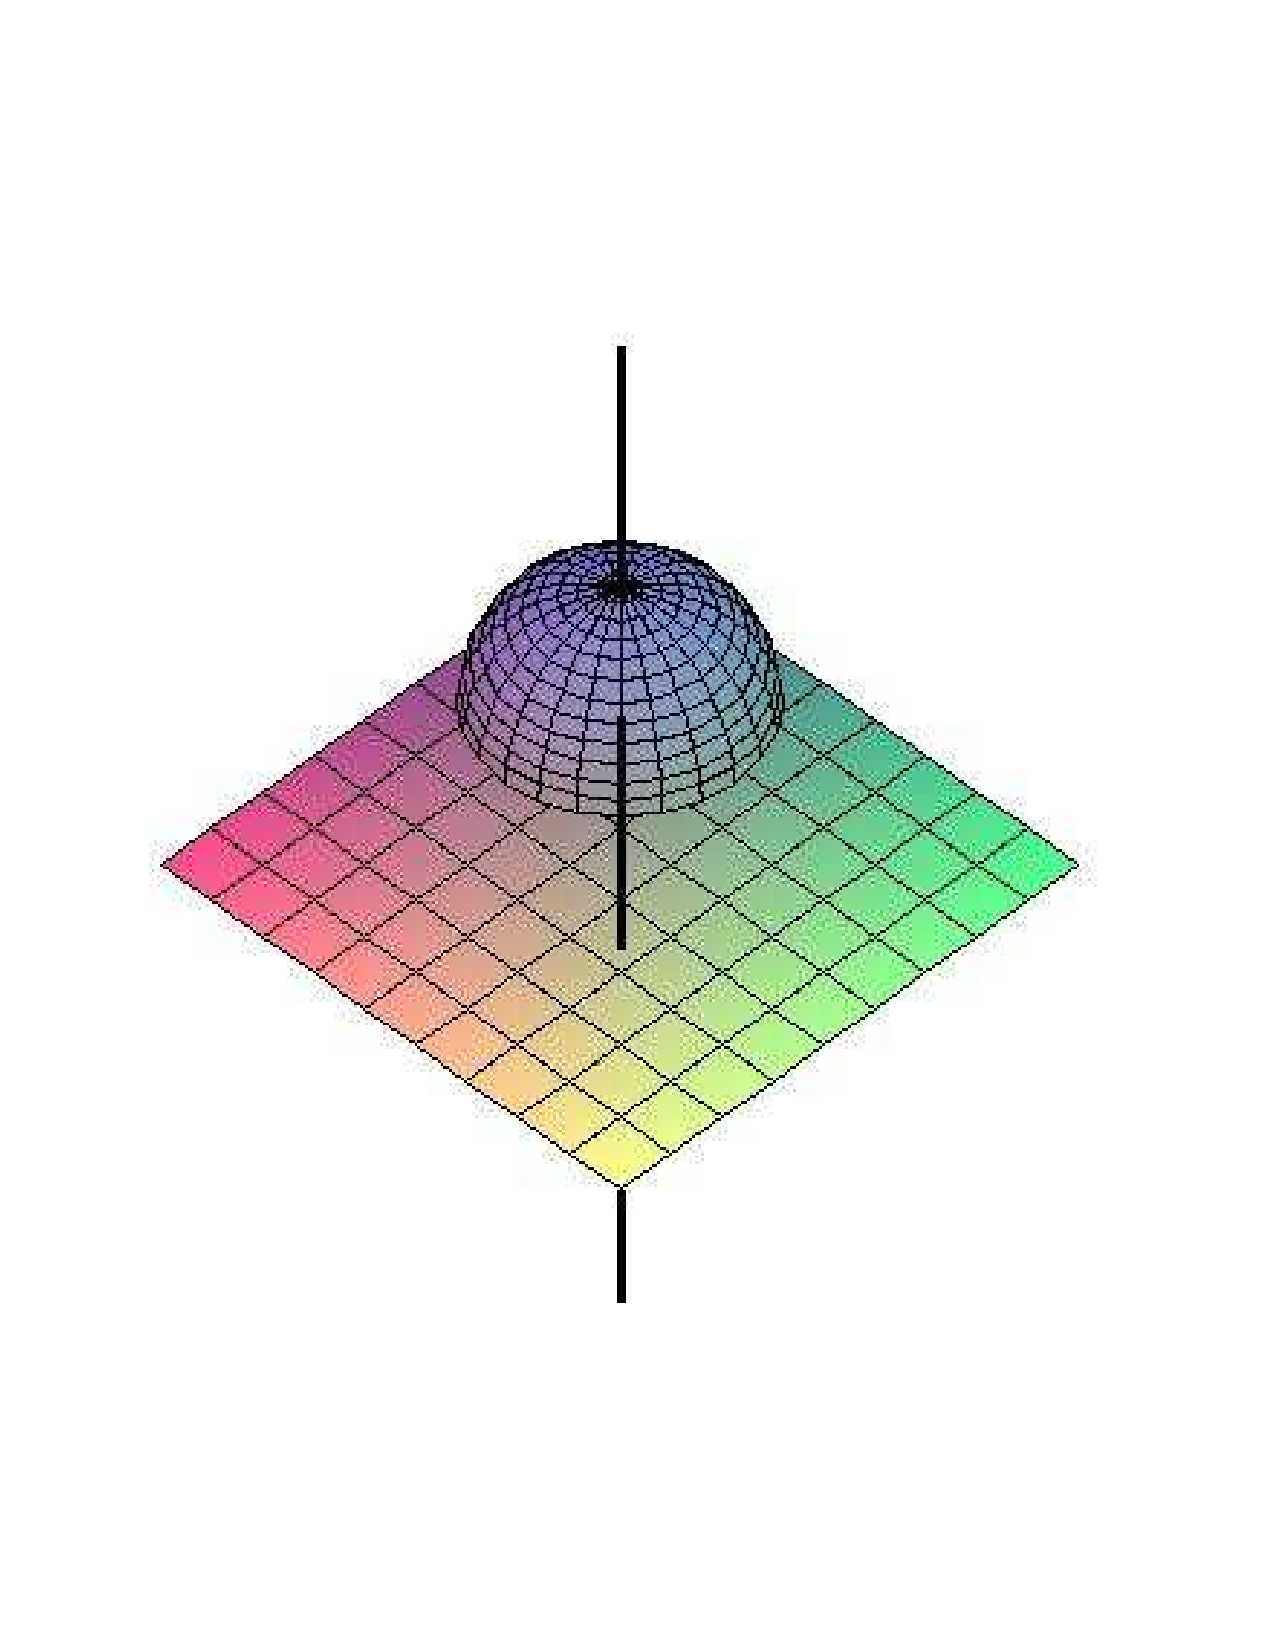
\includegraphics[width=8cm]{Ericatti_1.pdf}
 % Ericatti_1.pdf: 612x792 pixel, 72dpi, 21.59x27.94 cm, bb=0 0 612 792
 \caption{Projection stéréographique}
 \label{fig:Ericatti_1}
\end{figure}
Dans un espace orienté $\mathcal E$ muni d'un repère orthonormé direct $(O,\overrightarrow i,\overrightarrow j,\overrightarrow k)$, on note $N$ le point de coordonnées $(0,0,1)$ et $\mathcal S$ la sphère de centre $O$ et de rayon $1$.\newline
Les fonctions coordonnées relatives à ce repère sont désignées par $x$, $y$, $z$. Le produit scalaire de deux vecteurs $\overrightarrow u$ et $\overrightarrow v$ sera noté  $(\overrightarrow u / \overrightarrow v)$.\newline
Soit $\mathcal P$ le plan d'équation $z=0$. Il est muni du repère $(O,\overrightarrow i,\overrightarrow j)$ ce qui permet de définir l'affixe complexe $w=x(W)+iy(W)$ d'un point $W$ de ce plan.
\begin{enumerate}
\item Pour chaque point $M\in \mathcal S-\{N\}$ de coordonnées $(\alpha,\beta,\gamma)$, on considère la droite $(NM)$ (voir figure \ref{fig:Ericatti_1}). Son intersection avec le plan $\mathcal P$ est formée d'un seul point noté $W$ d'affixe $w$ appelé le projeté stéréographique de $M$.
\begin{enumerate}
 \item  Montrer que $\gamma \neq 1$ et que $w = \dfrac{\alpha + i\beta}{1- \gamma}$.
Montrer que $w = \dfrac{1+\gamma}{\alpha -i\beta}$  si $(\alpha,\beta)\neq(0,0)$.
Dans quel cas peut-on avoir $(\alpha,\beta)=(0,0)$ ? 
\item Montrer que
\begin{align*}
 \alpha = \dfrac{\overline{w}+w}{|w|^2+1} & & 
\beta = i\dfrac{\overline{w}-w}{|w|^2+1} & & 
\gamma =  \dfrac{|w|^2-1}{|w|^2+1}
\end{align*}
\item Préciser $\frac{\gamma}{1-\gamma}$ et $\frac{\beta}{1-\gamma}$ en fonction de $w$, $\overline{w}$ et $i$.
\end{enumerate}
\end{enumerate}
Dans la suite de cette partie, $\overrightarrow\Omega$ est un vecteur fixé de coordonnées $(p,q,r)$. On considère une courbe paramétrée définie dans un intervalle $I$ de $\R$
\begin{displaymath}
 \begin{aligned}
  I &\rightarrow \mathcal E\\
  t &\rightarrow M(t)
 \end{aligned}
\end{displaymath}
et à valeurs \emph{dans l'espace} $\mathcal E$. Pour chaque $t\in I$, les coordonnées de $M(t)$ sont $(\alpha(t),\beta(t),\gamma(t))$. Ainsi $\alpha$, $\beta$, $\gamma$ sont des fonctions de $I$ dans $\R$.\\
On suppose que cette courbe paramétrée est dérivable et vérifie
\begin{displaymath}
 \forall t\in I : \overrightarrow{M'}(t) = \overrightarrow{\Omega} \wedge \overrightarrow{OM(t)}
\end{displaymath}

\begin{enumerate} \setcounter{enumi}{1}
 \item Montrer que $\Vert \overrightarrow{OM(t)}\Vert$ et $(\overrightarrow \Omega / \overrightarrow{OM(t)})$ sont indépendantes de $t$. Que peut-on en déduire pour l'ensemble des points $M(t)$ ?

\item On considère un repère orthonormé direct
\begin{displaymath}
 (O,\overrightarrow I ,\overrightarrow J , \overrightarrow K) \text{ avec }
\overrightarrow K = 
\dfrac{1}{\Vert\overrightarrow{\Omega} \Vert}\overrightarrow{\Omega}
\end{displaymath}
Les coordonnées de $M(t)$ dans ce repère sont notées $(X(t),Y(t),Z(t))$. Former le système d'équations différentielles vérifiées par $X$, $Y$, $Z$. 
%??? On peut faire calculer explicitement en choissisant le repère tel que pour un $t_0$, $X(t_0)=\sqrt{1-\gamma_0^2}$, %$Y(t_0)=0$, $Z(t_0)=\gamma_0)$. ???
\item On suppose que pour tous les $t$ de $I$, $M(t)\in\mathcal S-\{N\}$. On note $w(t)$ l'affixe complexe du projeté stéréographique de $M(t)$.
\begin{enumerate}
 \item Vérifier que
\begin{displaymath}
 w'(t) = \dfrac{\alpha'(t)+i\beta'(t)+w(t)\gamma'(t)}{1-\gamma(t)}
\end{displaymath}
\item Vérifier que
\begin{multline*}
 \alpha'(t)+i\beta'(t)+w(t)\gamma'(t) \\= 
ir(\alpha(t)+i\beta(t))+(q-ip)\gamma(t)-w(t)q(\alpha +i\beta)+w(t)(p+iq)\beta(t)
\end{multline*}
\item En déduire les nombres complexes $a$, $b$, $c$ tels que
\begin{displaymath}
 w'(t) = a + bw(t) +cw^2(t)
\end{displaymath}
Cette relation est une forme particulière de l'équation différentielle dite \emph{de Ricatti}. Pour quelles valeurs de $p$, $q$, $r$ retrouve-t-on l'équation $(1)$ ?
\end{enumerate}

\end{enumerate}

